\documentclass[spanish,notes=hide]{beamer}

%Para crear una versión 'handout' (Copyright: Diego Berrueta)
%\documentclass[handout,notes=show]{beamer}

\usetheme{Warsaw}
\usepackage{beamerthemesplit}

\usepackage[spanish]{babel}
\usepackage[utf8]{inputenc}
\usepackage{listings}
\usepackage{graphicx}
\usepackage{colortbl}

\title{SWAML}
\subtitle{Publicaci\'on de listas de correo en Web Sem\'antica}
\author{Sergio Fern\'andez L\'opez}
\institute{%
	\href{http://swaml.berlios.de/}{http://swaml.berlios.de/}\\
	\vspace{0.7cm}
	Proyecto Fin de Carrera\\
	E.U. de Ingenier\'ia T\'ecnica en Inform\'atica de Oviedo
}
\date{20 de Diciembre de 2006}

\begin{document}

\frame{
  \note[item]{Saludar}
  \note[item]{Presentarse}
  \note[item]{Esta es la presentación del proyecto
    \textit{SWAML, publicación de listas de correo en Web Semántica}
  }

  \titlepage
}

%\frame{\tableofcontents}

\section{Introducción}

\subsection{Situación actual}
\frame
{
  \frametitle{Publicación actual de los archivos de listas de correo}

  \begin{itemize}
   \item<1-> Miles de listas de correo de las más variopinta temática
   \item<2-> Publicación en HTML de los archivos antiguos
   \item<3-> Pérdida de toda posibilidad de recuperar esa información
  \end{itemize}
}

\subsection{Objetivos}
\frame
{
  \frametitle{Objetivos}

  \begin{itemize}
   \item<1-> Objetivo principal: 
     \begin{itemize}
      \item \textbf{Publicación de los archivos antiguos de listas de correo en un formato rico semánticamente.}
     \end{itemize}
   \item<2-> Varios objetivos secundarios:
     \begin{itemize}
	\item Maximizar la reutilización de la infraestructura disponible previamente.
	\item Desarrollar un prototipo capar de recomponer listas de correo \textit{atacando} colecciones de ficheros RDF.
	\item Abrir la puerta a nuevas aplicaciones.
     \end{itemize}
  \end{itemize}
}

\subsection{La Web Semántica}
\frame
{
  \frametitle{Introducción a la Web Semántica}

  FIXME
}

\section{El proyecto SWAML}

\subsection{Tecnologías implicadas}
\frame
{
  \frametitle{RDF}

  FIXME
}
\frame
{
  \frametitle{SIOC}

  FIXME
}
\frame
{
  \frametitle{Python}

  FIXME
}

\subsection{Meollo}
\frame
{
  \frametitle{Meollo}

  FIXME
}

\section{Conclusiones}
\subsection{Resultados}
\frame
{
  FIXME\\
  aportación a SIOC
}
\subsection{Futuras líneas de trabajo}
\frame
{
  \frametitle{Futuro inmediato}

  \note[item]{ Usar GMail como fuente de información. }
  \note[item]{ Bastará disponer de una (o varias) cuentas de GMail suscritas a diferentes
    listas de correo. Después apenas habrá que optimizar el software para
    hacer más eficientes estas exportaciones automáticas. }
  \note[item]{ Esperamos llevar a cabo el experimento en la sproximas semanas. }

  \bigskip
  \begin{columns}
   \begin{column}{0.7\textwidth}
    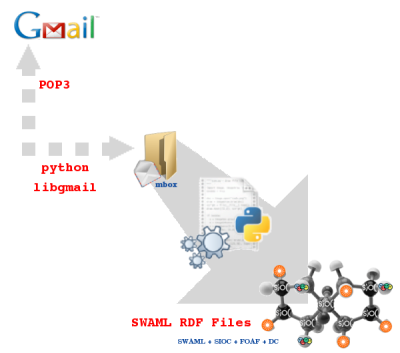
\includegraphics[width=0.99\textwidth]{images/gmail-swaml.png}
   \end{column}
   \begin{column}{0.4\textwidth}
    Automatizar el experimento aislado ya realizado por John Breslin:
    \begin{enumerate}
     \item Descargar los correos (\texttt{python-libgmail})
     \item Generar un mbox
     \item Usar SWAML para generar su descripción en RDF
    \end{enumerate}
   \end{column}
  \end{columns}
  \bigskip
}
\frame
{
  \frametitle{Futuro a medio plazo}
  \begin{itemize}
   \item Marcado semántico para el cuerpo de los mensajes
   \item API en Python para SIOC
   \item Integración con Mailman
   \item API para DIG
  \end{itemize}
}

\section{Demostración}
\subsection{Demostración}
\frame
{
  \note[item]{Crear una configuración en directo con asistente.}
  \note[item]{Ejemplo de exportación con SWAML (con todas las opciones), enseñar los RDF en plano.}
  \note[item]{Mismo ejemplo si enriquecer con FOAF ni exportación a KML.}
  \note[item]{Enriquecer con FOAF.}
  \note[item]{Exportar a KML.}
  \note[item]{Visualizarla con Buxon.}

  \begin{center}
    \LARGE{\textbf{demostración práctica}}
  \end{center}
}
\subsection{Preguntas}
\frame
{
  \note[item]{Agradecer la atención prestada.}
  \note[item]{Quedar a disposición del tribunal para contestar a las
		preguntas o ampliar cualquiera de los temas expuestos.}

  \begin{center}
    \LARGE{\textbf{¿preguntas?}}\\
    \vspace{3cm}
    \small{%
	Esta presentación se distribuye bajo los términos de la licencia
	CreativeCommons Reconocimiento-CompartirIgual 2.5
    }
  \end{center}
}

\appendix

\section{Respuestas preparadas}
\frame{
  FIXME: retocarlas según el tribunal
}


\end{document}
